% This example uses the 'minted' package, so you need to run the compiler with
% the '-shell-escape' option, i.e.
% 	pdflatex -shell-escape example.tex
% Additionally, you must have the 'pygmentize' program installed, which is part of
% the 'Pygments' package (https://pygments.org/)

\documentclass[aspectratio=1610, polish]{beamer}

% Jeśli chcesz otrzymać prezentację w języku polskim, to, powyżej, zamień „english” na „polish”
\usepackage{animate}
\usepackage{mdframed}
\usepackage{graphicx}
\graphicspath{{figures/}{./}}
\usepackage{babel}
\makeatletter
\usepackage{polski}
\makeatother
\usepackage[utf8]{inputenc}
\usepackage{tikz}
\usetikzlibrary{shapes,arrows,fit,positioning} % Rozszerzenia TikZ
\usepackage{xcolor} % Kolory, w tym niestandardowe jak Dandelion
\usepackage{multicol} % Obsługa wielu kolumn
\usepackage{booktabs} % Ładne tabele (\toprule, \midrule, \bottomrule)
\usepackage{listings} % We want to put listings
\mode<beamer>{ 	% In the 'beamer' mode
	\definecolor{links}{HTML}{2A1B81}
	\hypersetup{
		pdfpagemode=FullScreen,                 % Enable Full screen mode
		colorlinks,
		linkcolor=,
		urlcolor=links
	}
	\usetheme[parttitle=rightfooter]{AGH}       % Show part title in right footer
	% \usetheme[nosidebar]{AGH}                  % Do not show sidebar on non-title slides
	%\usetheme[nosidebar, margins=1em]{AGH}     % Do not show sidebar on non-title slides and set both margins (left / right) to 1em
	% \usetheme[dark]{AGH}                       % Use dark background
	% \usetheme[dark, parttitle=leftfooter]{AGH} % Use dark background and show part title in left footer
}
\mode<handout>{	% In the 'handout' mode
	\hypersetup{pdfpagemode=None}
	\usepackage{pgfpages}
	\pgfpagesuselayout{4 on 1}[a4paper,border shrink=5mm,landscape]	% Show 4 slides on 1 page
	\pgfpageslogicalpageoptions{1}{border code=\pgfusepath{stroke}}
	\pgfpageslogicalpageoptions{2}{border code=\pgfusepath{stroke}}
	\pgfpageslogicalpageoptions{3}{border code=\pgfusepath{stroke}}
	\pgfpageslogicalpageoptions{4}{border code=\pgfusepath{stroke}}
  	\usetheme{boxes}
  	\addheadbox{structure}{\quad\insertpart\hfill\insertsection\hfill\insertsubsection\qquad}          % Content of header
 	\addfootbox{structure}{\quad\insertshortauthor\hfill\insertframenumber\hfill\insertsubtitle\qquad} % Content of footer
}

\AtBeginPart{ % At begin part: display its name
	\frame{\partpage}
}
\author[Kmąk, Miklas, Wójcik]{Maciej Kmąk \and Hubert Miklas \and Mateusz Wójcik}
\date{}
\title{Klasyfikacja obrazów metodami klasycznej wizji komputerowej}
\subtitle{Jabłka vs pomidory}
\institute[AGH]{
        Akademia Górniczo-Hutnicza \\
        Systemy Wizyjne
}
%%%%%%%%%%% Configuration of the listings package %%%%%%%%%%%%%%%%%%%%%%%%%%
% Source: https://en.wikibooks.org/wiki/LaTeX/Source_Code_Listings#Using_the_listings_package
%%%%%%%%%%%%%%%%%%%%%%%%%%%%%%%%%%%%%%%%%%%%%%%%%%%%%%%%%%%%%%%%%%%%%%%%%%%%
\lstset{ %
  backgroundcolor=\color{white},   % choose the background color
  basicstyle=\footnotesize,        % the size of the fonts that are used for the code
  breakatwhitespace=false,         % sets if automatic breaks should only happen at whitespace
  breaklines=true,                 % sets automatic line breaking
  captionpos=b,                    % sets the caption-position to bottom
  commentstyle=\color{green},      % comment style
  deletekeywords={...},            % if you want to delete keywords from the given language
  escapeinside={\%*}{*)},          % if you want to add LaTeX within your code
  extendedchars=true,              % lets you use non-ASCII characters; for 8-bits encodings only, does not work with UTF-8
  frame=single,	                   % adds a frame around the code
  keepspaces=true,                 % keeps spaces in text, useful for keeping indentation of code (possibly needs columns=flexible)
  keywordstyle=\color{blue},       % keyword style
  morekeywords={*,...},            % if you want to add more keywords to the set
  numbers=left,                    % where to put the line-numbers; possible values are (none, left, right)
  numbersep=5pt,                   % how far the line-numbers are from the code
  numberstyle=\tiny\color{gray},   % the style that is used for the line-numbers
  rulecolor=\color{black},         % if not set, the frame-color may be changed on line-breaks within not-black text (e.g. comments (green here))
  showspaces=false,                % show spaces everywhere adding particular underscores; it overrides 'showstringspaces'
  showstringspaces=false,          % underline spaces within strings only
  showtabs=false,                  % show tabs within strings adding particular underscores
  stepnumber=2,                    % the step between two line-numbers. If it's 1, each line will be numbered
  stringstyle=\color{cyan},        % string literal style
  tabsize=2,	                   % sets default tabsize to 2 spaces
  title=\lstname,                  % show the filename of files included with \lstinputlisting; also try caption instead of title
                                   % needed if you want to use UTF-8 Polish chars
  literate={ą}{{\k{a}}}1
           {Ą}{{\k{A}}}1
           {ę}{{\k{e}}}1
           {Ę}{{\k{E}}}1
           {ó}{{\'o}}1
           {Ó}{{\'O}}1
           {ś}{{\'s}}1
           {Ś}{{\'S}}1
           {ł}{{\l{}}}1
           {Ł}{{\L{}}}1
           {ż}{{\.z}}1
           {Ż}{{\.Z}}1
           {ź}{{\'z}}1
           {Ź}{{\'Z}}1
           {ć}{{\'c}}1
           {Ć}{{\'C}}1
           {ń}{{\'n}}1
           {Ń}{{\'N}}1
}

\begin{document}

\begin{frame}[t]
    \maketitle
\end{frame}

\begin{frame}{Plan prezentacji}
    \tableofcontents
\end{frame}

% ============================================================ %
\section{Wprowadzenie i zbiór danych}
% ============================================================ %
\begin{frame}{Cel projektu}
    \textbf{Zadanie:} klasyfikacja obrazów \emph{wyłącznie} metodami klasycznej
    wizji komputerowej i uczenia maszynowego -- bez sieci neuronowych.
    \pause
    \vspace{0.5cm}

    \textbf{Pipeline:}
    \begin{itemize}
        \item wczytanie danych,
        \item preprocessing (czyszczenie, segmentacja obiektu od tła),
        \item ekstrakcja cech (tekstura, kolor, kształt),
        \item klasyfikacja i dobór parametrów (podział train / walidacja),
        \item ocena na \emph{osobnym} zbiorze testowym.
    \end{itemize}
\end{frame}

\begin{frame}{Zbiór danych: jabłka vs pomidory}
    \begin{columns}[T]
        \begin{column}{0.52\textwidth}
            \begin{itemize}
                \item Owoce RGB, z gotowym podziałem na train/test.
                \item Trening: \textbf{164} jabłka, \textbf{130} pomidorów.
                \item Test: \textbf{54} jabłka, \textbf{43} pomidory.
            \end{itemize}
            \vspace{0.3cm}
            \pause
            \textbf{Dlaczego trudny?}
            \begin{itemize}
                \item Obie klasy bywają czerwone i okrągłe.
                \item Część zdjęć to kiście, owoce pokrojone, różne tła.
            \end{itemize}
        \end{column}
        \begin{column}{0.46\textwidth}
            \centering
            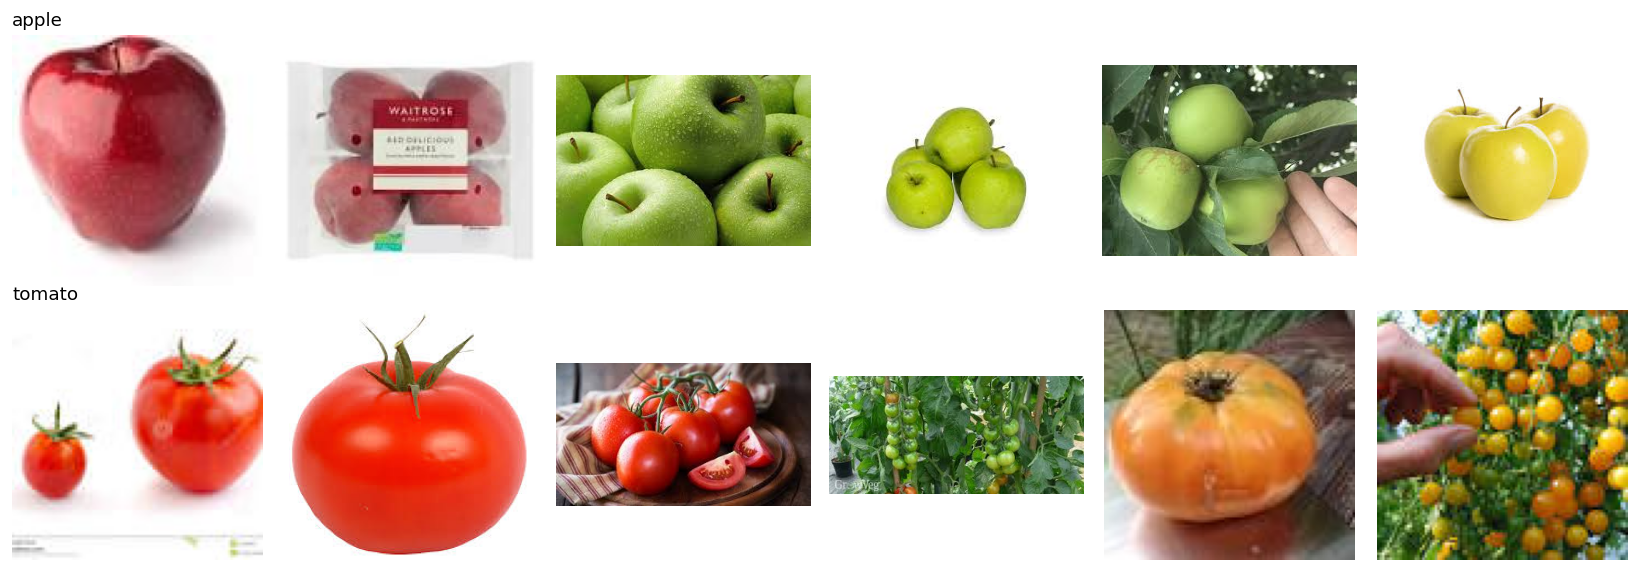
\includegraphics[width=\linewidth]{apple_tomato.png}
        \end{column}
    \end{columns}
\end{frame}

% ============================================================ %
\section{Preprocessing}
% ============================================================ %
\begin{frame}{Działanie preprocessingu}
    \begin{itemize}
        \item \textbf{Usunięcie artefaktów} -- filtr medianowy (szum „sól i
              pieprz", bloki JPEG; zachowuje krawędzie lepiej niż rozmycie Gaussa).
        \pause
        \item \textbf{Balans bieli} -- metoda \emph{gray-world}, redukcja
              dominującej barwy.
        \pause
        \item \textbf{Kontrast} -- CLAHE na kanale $L$ (LAB); barwa i nasycenie
              pozostają nietknięte.
        \pause
        \item \textbf{Segmentacja} -- progowanie w HSV + morfologia (otwarcie,
              domknięcie) + największa składowa spójna.
    \end{itemize}
    \vspace{0.2cm}
    \pause
    \centering
    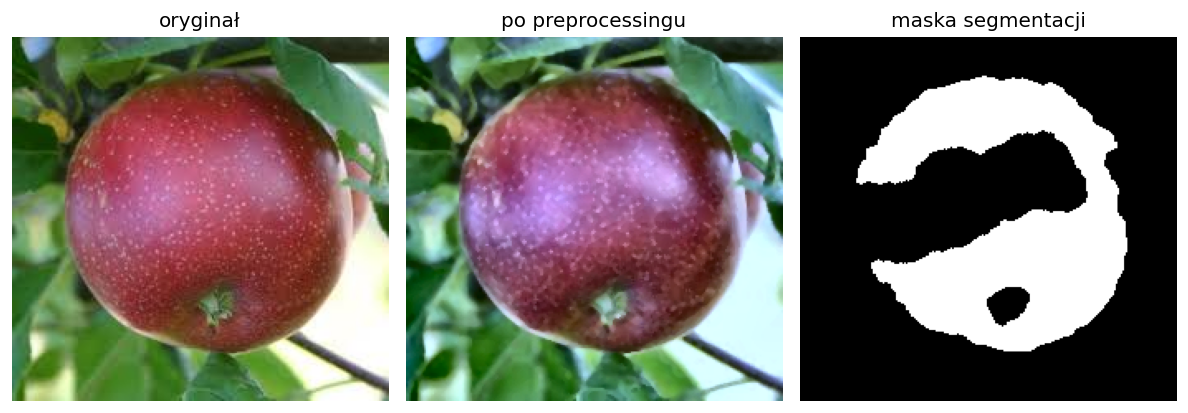
\includegraphics[width=0.78\linewidth]{preprocess.png}
\end{frame}

\begin{frame}{Dlaczego HSV, a nie Otsu?}
    \begin{itemize}
        \item Otsu progu­je po \textbf{jasności} -- rozpada się, gdy tło jest
              kolorowe lub zielone (np. pomidory na krzaku).
        \item HSV progu­je po \textbf{kolorze} (ciepłe barwy owoców) -- trzyma
              kształt owocu niezależnie od tła.
    \end{itemize}
    \vspace{0.5cm}
    \pause
    \begin{block}{Potwierdzenie liczbowe (ten sam zestaw cech, SVM)}
        \centering
        maska HSV: $F_1 = 0{,}747$ \qquad vs \qquad maska Otsu: $F_1 = 0{,}738$
    \end{block}
\end{frame}

\begin{frame}{Segmentacja -- Otsu vs HSV}
    \centering
    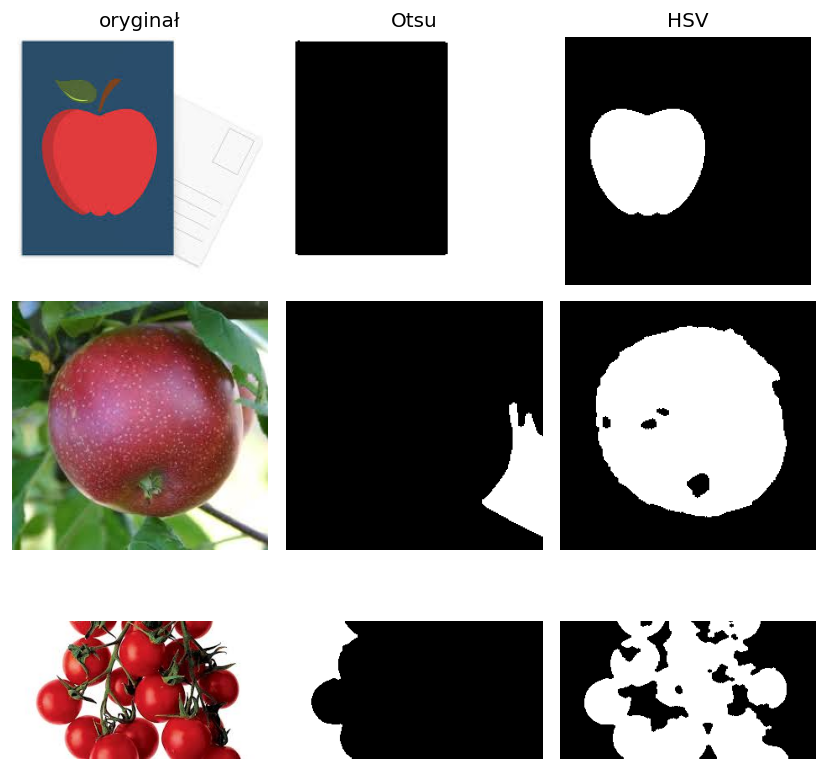
\includegraphics[width=0.7\linewidth]{segmentation.png}

    \vspace{0.2cm}
    {\footnotesize Otsu (po jasności) zawodzi na kolorowym/zielonym tle; HSV (po
    kolorze) izoluje owoc.}
\end{frame}

% ============================================================ %
\section{Ekstrakcja cech}
% ============================================================ %
\begin{frame}{Cechy -- 203 wartości na obraz}
    Liczone na masce obiektu, w trzech komplementarnych grupach. Preferujemy
    deskryptory niezmiennicze względem skali i obrotu.
    \vspace{0.3cm}
    \begin{itemize}
        \item \textbf{Tekstura (66):} macierz GLCM -- deskryptory Haralicka
              (kontrast, niepodobieństwo, jednorodność, energia, korelacja, ASM,
              entropia) -- oraz histogram lokalnych wzorców binarnych (LBP).
        \pause
        \item \textbf{Kolor (75):} dla RGB/HSV/Lab statystyki (średnia, odchylenie,
              skośność, mediana, kurtoza, kwartyle) + histogram odcienia.
        \pause
        \item \textbf{Kształt (62):} geometria konturu, momenty Hu, deskryptory
              Fouriera, wymiar fraktalny, miary otoczki wypukłej, momenty Zernike'a.
    \end{itemize}
\end{frame}

% ============================================================ %
\section{Klasyfikacja i dobór parametrów}
% ============================================================ %
\begin{frame}{Modele i strojenie}
    \textbf{Pięć klasycznych klasyfikatorów} (\texttt{scikit-learn}): SVM, drzewo
    decyzyjne, las losowy, $k$-NN oraz regresja logistyczna.
    \vspace{0.4cm}
    \begin{itemize}
        \item Każdy w potoku \texttt{StandardScaler} + klasyfikator -- skalowanie
              uczone tylko na foldzie treningowym (brak wycieku informacji).
        \pause
        \item Hiperparametry: \texttt{GridSearchCV}, walidacja krzyżowa
              stratyfikowana, metryka $F_1$ makro.
        \pause
        \item Podział: trening (z walidacją) do strojenia i wyboru modelu,
              \textbf{osobny zbiór testowy} tylko do oceny końcowej.
    \end{itemize}
\end{frame}

% ============================================================ %
\section{Wyniki i analiza}
% ============================================================ %
\begin{frame}{Wyniki na zbiorze testowym}
    \centering
    \begin{table}\small
    \begin{tabular}{lcccc}
        \toprule
        Model & Accuracy & Precyzja & Czułość & $F_1$ \\
        \midrule
        \textbf{kNN}      & \textbf{0,814} & 0,815 & 0,807 & \textbf{0,810} \\
        Drzewo decyzyjne  & 0,773 & 0,779 & 0,761 & 0,764 \\
        Regresja log.     & 0,763 & 0,775 & 0,747 & 0,750 \\
        Las losowy        & 0,753 & 0,751 & 0,745 & 0,747 \\
        SVM               & 0,753 & 0,761 & 0,738 & 0,740 \\
        \bottomrule
    \end{tabular}
    \end{table}
    \footnotesize (średnie makro)
    \vspace{0.3cm}
    \pause

    \normalsize Najlepszy \textbf{kNN}: accuracy \textbf{0,814}, $F_1$ makro
    \textbf{0,810} -- znacznie powyżej poziomu bazowego klasy większościowej
    ($0{,}557$).
\end{frame}

\begin{frame}{Gdzie model się myli}
    \begin{columns}[T]
        \begin{column}{0.48\textwidth}
            \centering
            \begin{table}\small
            \begin{tabular}{lcc}
                \toprule
                Prawda\,$\backslash$\,Pred. & jabłko & pomidor \\
                \midrule
                jabłko  & 47 & 7 \\
                pomidor & 11 & 32 \\
                \bottomrule
            \end{tabular}
            \end{table}
        \end{column}
        \begin{column}{0.5\textwidth}
            \begin{itemize}
                \item Jabłka: czułość $0{,}87$ (47/54).
                \item Pomidory: czułość $0{,}74$ (32/43).
                \item Błędy idą w obie strony -- klasy mocno się nakładają (widać
                      to też na rzucie PCA).
            \end{itemize}
        \end{column}
    \end{columns}
\end{frame}

\begin{frame}{Co napędza klasyfikację?}
    Sprawdziliśmy dwiema metodami: ważnością cech (Random Forest) i ablacją
    rodzin (ten sam model, zmieniany tylko zestaw cech).
    \vspace{0.3cm}
    \begin{columns}[T]
        \begin{column}{0.5\textwidth}
            \textbf{Ablacja ($F_1$ w CV):}
            \begin{itemize}
                \item wszystko: \textbf{0,785}
                \item tekstura: 0,757
                \item kolor: 0,715
                \item kształt: 0,675
            \end{itemize}
        \end{column}
        \begin{column}{0.5\textwidth}
            \textbf{Ważność (Random Forest):}
            \begin{itemize}
                \item tekstura (GLCM): 0,45
                \item kolor: 0,26
                \item pozostałe: $\le 0{,}07$
            \end{itemize}
        \end{column}
    \end{columns}
    \vspace{0.3cm}
    \pause
    \centering
    \emph{Tekstura niesie najwięcej, kolor jest drugi, kształt mało -- a pełny
    zestaw cech wygrywa.}
\end{frame}

\begin{frame}{Wkład rodzin cech -- wykresy}
    \begin{columns}[c]
        \begin{column}{0.5\textwidth}
            \centering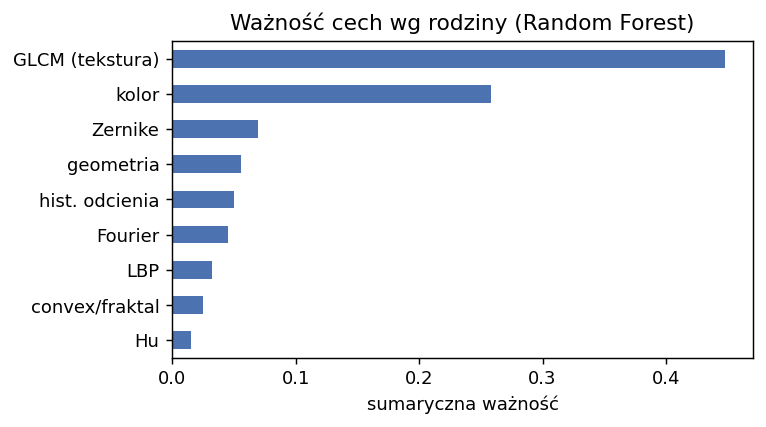
\includegraphics[width=\linewidth]{feat_importance.png}
        \end{column}
        \begin{column}{0.5\textwidth}
            \centering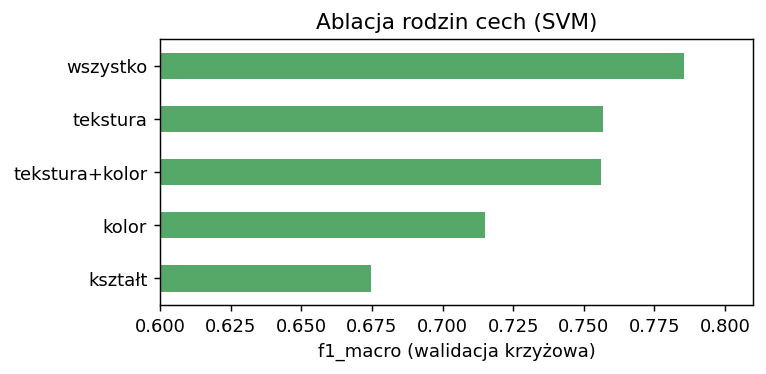
\includegraphics[width=\linewidth]{ablation.png}
        \end{column}
    \end{columns}
    \vspace{0.2cm}
    \centering {\footnotesize Tekstura i kolor dominują; pełny zestaw cech wygrywa.}
\end{frame}

\begin{frame}{Dlaczego to trudne -- rzut PCA}
    \centering
    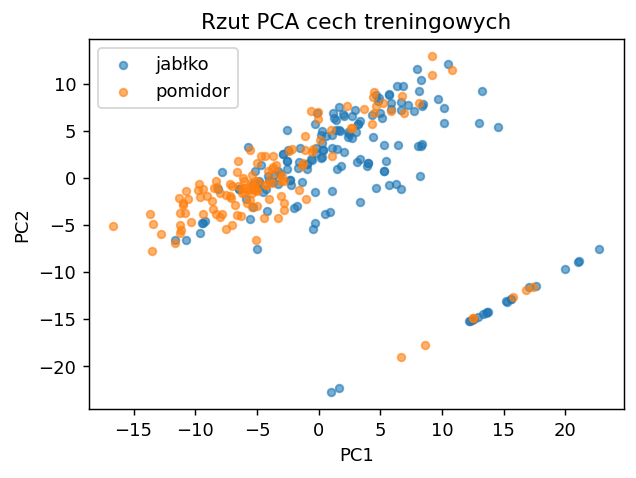
\includegraphics[width=0.56\linewidth]{pca.png}

    \vspace{0.2cm}
    {\footnotesize Klasy mocno się nakładają -- to ogranicza górną granicę metod
    klasycznych.}
\end{frame}

% ============================================================ %
\section{Wnioski}
% ============================================================ %
\begin{frame}{Wnioski}
    \begin{itemize}
        \item Klasyczny potok klasyfikuje jabłka i pomidory z accuracy
              $0{,}814$ i $F_1$ makro $0{,}810$ (baseline $0{,}557$).
        \pause
        \item Najwięcej wnoszą \textbf{tekstura} (gładki, błyszczący pomidor vs
              matowe jabłko) i \textbf{kolor}; kształt mało -- oba owoce są okrągłe.
        \pause
        \item \textbf{Segmentacja po kolorze (HSV)} bije Otsu i jest kluczowa dla
              jakości cech koloru i kształtu.
        \pause
        \item Ograniczeniem jest sam zbiór: nakładające się klasy, kiście, owoce
              pokrojone i różne tła.
    \end{itemize}
\end{frame}

\begin{frame}{Dygresja: czy ten zbiór jest na pewno poważny?}
    \centering Cztery autentyczne „perełki” ze zbioru:
    \vspace{0.15cm}
    \begin{columns}[T]
        \begin{column}{0.24\textwidth}\centering
            \includegraphics[width=\linewidth,height=2.7cm,keepaspectratio]{grucha.png}\\
            {\scriptsize Czapetka (\emph{java apple})}
        \end{column}
        \begin{column}{0.24\textwidth}\centering
            \includegraphics[width=\linewidth,height=2.7cm,keepaspectratio]{owad.png}\\
            {\scriptsize Owad jako „pomidor”?}
        \end{column}
        \begin{column}{0.24\textwidth}\centering
            \includegraphics[width=\linewidth,height=2.7cm,keepaspectratio]{whois.png}\\
            {\scriptsize \href{https://veggietales.fandom.com/wiki/Joe}{Who is Joe?}}
        \end{column}
        \begin{column}{0.24\textwidth}\centering
            \includegraphics[width=\linewidth,height=2.7cm,keepaspectratio]{ogor.jpeg}\\
            {\scriptsize \href{https://www.youtube.com/watch?v=j4Ph02gzqmY}{Ogór}}
        \end{column}
    \end{columns}
    \vspace{0.2cm}
    \pause
    \begin{block}{Pytanie pozostawimy otwartym}
        Skoro w klasie \emph{apple} mieści się nawet czapetka (\emph{java apple}),
        to czemu w zbiorze nie ma \emph{pineapple}, skoro też ma „apple” w nazwie?
    \end{block}
\end{frame}

\begin{frame}{}
    \centering \Huge
    \emph{Dziękujemy za uwagę!}
\end{frame}

\end{document}
